% Cread by Banbara on Dec. 19 2019
\documentclass[11pt,dvipdfmx,handout]{beamer}

%\documentclass[a4paper,12pt]{jarticle}
%\usepackage{beamerarticle}

%%%% Packages %%%%%
 \usepackage{graphicx}
% \usepackage{amsmath,amssymb,amsthm}
% \usepackage{multirow}
% \usepackage{url}
% \usepackage{tikz}
% \usepackage{alltt}
\usepackage{bm}
% \usepackage{listings,jlisting}
% \usepackage{listings}
% \lstset{
%  basicstyle=\ttfamily\scriptsize,
%  keepspaces=true,
%  escapechar=|,
%  columns=[l]{fullflexible}
% }
\usepackage{tikz}
\usetikzlibrary{positioning}

%%%% Fonts %%%%%
\renewcommand{\kanjifamilydefault}{\gtdefault}
% \usepackage{otf} % otfパッケージ
\usepackage[deluxe]{otf} 
\usepackage{txfonts} % 数式・英文ローマン体を Lxfont にする
% \usepackage[T1]{fontenc} % 8bit フォント
% \usepackage{minijs}
% \usepackage{textcomp} % 欧文フォントの追加
% \usepackage[utf8]{inputenc} % 文字コードをUTF-8

%%%% Beamer %%%%%
\usetheme{Madrid}
\useinnertheme{rectangles}
%\useoutertheme{smoothbars}
\setbeamercolor{enumerate}{fg=white, bg=black}
\usefonttheme{professionalfonts}
\setbeamertemplate{frametitle}[default][center]
\setbeamertemplate{navigation symbols}{}
% \setbeamercovered{transparent} % 好みに応じてどうぞ
\setbeamertemplate{footline}[frame number]
\setbeamercolor{page number in head/foot}{fg=black} % ページ数を表示する
\setbeamertemplate{navigation symbols}{}
\newcommand{\backupbegin}{
   \newcounter{framenumberappendix}
   \setcounter{framenumberappendix}{\value{framenumber}}
}
\newcommand{\backupend}{
   \addtocounter{framenumberappendix}{-\value{framenumber}}
   \addtocounter{framenumber}{\value{framenumberappendix}} 
}% ページ表示(補助スライドを除く)
\usepackage{appendixnumberbeamer}
% \setbeamerfont{footline}{size=\normalsize,series=\bfseries}
\setbeamerfont{footline}{size=\scriptsize,series=\mdseries}
\setbeamercolor{footline}{fg=black,bg=black}
\setbeamertemplate{blocks}[rounded][shadow=true]
\setbeamertemplate{items}[ball]
% \setbeamertemplate{enumerate items}[default]
% \setbeamerfont{alerted text}{series=\bfseries}

%%%% My macro %%%%%
%%%%%%%%%%%%%%%%%%%%%%%%%%%%%%%%%%%%%%%%%%%%%%%%%%%%%%%%%%%%%%%%
% User-defined Macro
%%%%%%%%%%%%%%%%%%%%%%%%%%%%%%%%%%%%%%%%%%%%%%%%%%%%%%%%%%%%%%%%
\newcommand{\compress}{\itemsep0pt\parsep0pt\parskip0pt\partopsep0pt}
% \newcommand{\compress}{\itemsep1pt plus1pt\parsep0pt\parskip0pt}
% \newcommand{\code}[1]{\lstinline[basicstyle=\ttfamily]{#1}}
\newcommand{\gringo}{\textit{gringo}}
\newcommand{\clasp}{\textit{clasp}}
\newcommand{\clingo}{\textit{clingo}}
\newcommand{\teaspoon}{\textit{teaspoon}}
\newcommand{\sat}{\textsf{SAT}}
\newcommand{\unsat}{\textsf{UNSAT}}
% \newcommand{\web}[2]{\href{#1}{#2\ \raisebox{-0.15ex}{\beamergotobutton{Web}}}}
% \newcommand{\doi}[2]{\href{#1}{#2\ \raisebox{-0.15ex}{\beamergotobutton{DOI}}}}
% \newcommand{\weblink}[1]{\web{#1}{#1}}
% \newcommand{\imp}{\mathrel{\Rightarrow}}
% \newcommand{\Iff}{\mathrel{\Leftrightarrow}}
% \newcommand{\mybox}[1]{\fbox{\rule[.2cm]{0cm}{0cm}\mbox{${#1}$}}}
% \newcommand{\mycbox}[2]{\tikz[baseline]\node[fill=#1!10,anchor=base,rounded corners=2pt] () {#2};}
% \newcommand{\naf}[1]{\ensuremath{{\sim\!\!{#1}}}}
% \newcommand{\head}[1]{\ensuremath{\mathit{head}(#1)}}
% \newcommand{\body}[1]{\ensuremath{\mathit{body}(#1)}}
% \newcommand{\atom}[1]{\ensuremath{\mathit{atom}(#1)}}
% \newcommand{\poslits}[1]{\ensuremath{{#1}^+}}
% \newcommand{\neglits}[1]{\ensuremath{{#1}^-}}
% \newcommand{\pbody}[1]{\poslits{\body{#1}}}
% \newcommand{\nbody}[1]{\neglits{\body{#1}}}
% \newcommand{\Cn}[1]{\ensuremath{\mathit{Cn}(#1)}}
% \newcommand{\reduct}[2]{\ensuremath{#1^{#2}}}
% \newcommand{\OK}{\mbox{\textcolor{green}{\Pisymbol{pzd}{52}}}}
% \newcommand{\KO}{\mbox{\textcolor{red}{\Pisymbol{pzd}{56}}}}
% \newcommand{\code}[1]{\lstinline[basicstyle=\ttfamily]{#1}}
% \newcommand{\lw}[1]{\smash{\lower2.ex\hbox{#1}}}
\newcommand{\llw}[1]{\smash{\lower3.ex\hbox{#1}}}

\newenvironment{tableC}{%
  \scriptsize
  \renewcommand{\arraystretch}{0.9}
  \tabcolsep = 0.6mm
  % \begin{tabular}[t]{p{6mm}|rlr|rlr|rlr|rlr|rlr}\hline
  %   \multicolumn{1}{l|}{\llw{問題   }} &
  \begin{tabular}[t]{l|rlr|rlr|rlr|rlr|rlr}\hline
    \multicolumn{1}{l|}{\llw{問題}} &
    \multicolumn{3}{c|}{UD1} &
    \multicolumn{3}{c|}{UD2} &
    \multicolumn{3}{c|}{UD3} &
    \multicolumn{3}{c|}{UD4} &
    \multicolumn{3}{c}{UD5} \\
    & 
    \multicolumn{1}{c}{既知の} & & \multicolumn{1}{c|}{ASP} & 
    \multicolumn{1}{c}{既知の} & & \multicolumn{1}{c|}{ASP} & 
    \multicolumn{1}{c}{既知の} & & \multicolumn{1}{c|}{ASP} & 
    \multicolumn{1}{c}{既知の} & & \multicolumn{1}{c|}{ASP} & 
    \multicolumn{1}{c}{既知の} & & \multicolumn{1}{c}{ASP} \\
    & 
    ベスト & &  & 
    ベスト & &  & 
    ベスト & &  & 
    ベスト & &  & 
    ベスト & &  \\
    \hline
  }{%
    \hline
  \end{tabular}
}

%%%%%%%%%%%%%%%%%%%%%%%%%%%%%%%%%%%%%%%%%%%%%%%%%%%%%%%%%%%%%%%%%%%%%%%
\title{解集合プログラミングに基づく\\系統的探索と確率的局所探索の統合的手法}
\author{桑原 和也}
%\institute{名古屋大学工学部電気電子・情報学科情報コース}
\date{2020年度中間発表\\2021年2月24日}
\institute{番原研究室}
\begin{document}
\maketitle
%%%%%%%%%%%%%%%%%%%%%%%%%%%%%%%%%%%%%%%%%%%%%%%%%%%%%%%%%%%%%%%%%%%%%%%
\begin{frame}{解集合プログラミング(Answer Set Programming; ASP)}
  \begin{itemize}
  \item \structure{\bf ASP言語}は,一階論理に基づく宣言的知識表現言語である.
  \item \structure{\bf ASPソルバー}は,安定モデル意味論~[Gelfond and Lifschitz '88]
    に基づく解集合を計算するプログラムである.
  \item 応用の一つとして,時間割問題などの求解困難な組合せ最適化問題に対し,
  未解決問題の最適値決定に成功している.
  \end{itemize}
  \begin{alertblock}{組合せ最適化問題に対してASPを用いる利点}
    \begin{itemize}
 %   \item ASP言語の高い表現力により,各制約を表現する論理プログラムを
 %    モジュール化して容易に切り替え可能である.
    \item ASP言語の高い表現力により,記号的制約を簡潔に記述できる.
    \item 系統的探索 (分枝限定法) なので,解の最適性を保証できる.
%    \item 様々な最適化手法や探索ヒューリスティックスを試せる.
    \item 探索ヒューリスティクスを試せる.
      \begin{itemize}
      \item 探索時に優先的に割り当てる値を指定できる.
      \end{itemize}
    \item API を利用して,メタヒューリスティクスを実装できる.
    \end{itemize}
  \end{alertblock}
\end{frame}
%%%%%%%%%%%%%%%%%%%%%%%%%%%%%%%%%%%%%%%%%%%%%%%%%%%%%%%%%%%%%%%%%%%%%%%
\begin{frame}{時間割問題}
  \begin{block}{}\centering
    求解困難な組合せ最適化問題の一種である.
  \end{block}
  \begin{itemize}
    % \item 現状では,実行可能で質の高い時間割を作成するために
    %   多くの人間の労力が費やされている.
  \item 時間割に関する国際会議 PATAT および
    \alert{\bf 国際的な時間割競技会}が開催され,
    時間割ソルバーの性能向上に貢献している.
    \begin{itemize}
    \item 教育時間割
      \begin{itemize}
      \item \alert{\bf カリキュラムベース・コース時間割 (CB-CTT)}
      \item ポストエンロールメント・コース時間割
      \item 試験時間割
      \end{itemize}
    \item 輸送時間割
    \item 従業員時間割
    \item スポーツ時間割
    \end{itemize}
  %\item 本発表では,最も研究が盛んな CB-CTT を対象とする.
  \begin{block}{カリキュラムベース・コース時間割 (CB-CTT)}
  %\item CB-CTT は,以下のように定式化される.
    \begin{itemize}
    \item 必ず満たすべき\structure{\bf ハード制約}と, 
    できるだけ満たしたい\structure{\bf 重み付きソフト制約}から構成される.
    \item 違反するソフト制約の重み (ペナルティ) の総和の最小化が目的.
    \end{itemize}
   \end{block}
  \end{itemize}
\end{frame}
%%%%%%%%%%%%%%%%%%%%%%%%%%%%%%%%%%%%%%%%%%%
\begin{frame}{ASPの研究における問題点}
  \begin{itemize}
  \item ASP による CB-CTT の解法は,
    最も成功した ASP 応用事例の一つとして知られている~[Banbara+ '13, '16, '18].
    \begin{itemize}
    \item ベンチマーク問題305問のうち,
      182問で既知の最良値と同じかより良い値が求められている.
  \item %系統的探索であることを活かして,
  最適値が未知であった51問の問題で最適値決定にも成功している.
 %   \begin{itemize}
 %   \item 305問中51問で最適値が求められている.
 %   \end{itemize}
     \end{itemize}
  \begin{alertblock}{既存ASP解法の問題点}
    \begin{itemize}
    \item %系統的探索をベースにしたものであり,
    ソフト制約が多く含まれるような問題集において,
      局所的探索より性能が劣っている場合がみられる.
     \item 既知の最良値との比の平均値は
       \begin{itemize}
       \item ソフト制約が少ない問題集 (UD1) では $+19.83\%$
       \item ソフト制約が多い問題集 (UD5) では $+100.17\%$
       \end{itemize}
    \end{itemize}
  \end{alertblock}
  \begin{block}{}\centering
   問題規模に対するスケーラビリティに限界がある.
  \end{block}
  \end{itemize}
\end{frame}
%%%%%%%%%%%%%%%%%%%%%%%%%%%%%%%%%%%%%%%%%%%%%%%%%%%%%%%%%%%%%%%%%%%%%%%
\begin{frame}{研究概要}
 \begin{alertblock}{研究目的}
    ASP 技術を用いて,
   系統的探索と確率的局所探索を統合的かつ効率的に
   扱う探索手法およびソルバーの実現を目指す.
 \end{alertblock}

 \begin{exampleblock}{研究の方針}
  \begin{itemize}
  \item 近似解法の一種である
  \alert{巨大近傍探索} (Large Neighborhood Search; LNS) [Pisinger 2010]に
  着想を得た,
  \alert{優先度付き巨大近傍探索} (Large Neighborhood Prioritized Search; LNPS) [坡山'18]
  をベースに探索手法に関する研究開発を進める.
  \item 時間割問題等の重要な応用研究を通じて,
  提案手法およびソルバーを評価する.
  \end{itemize}
 \end{exampleblock}
\end{frame}
%%%%%%%%%%%%%%%%%%%%%%%%%%%%%%%%%%%%%%%%%%%%%%%%%%%%%%%%%%%%%%%%%%%%%%%
\begin{frame}{研究概要}
 \begin{block}{研究内容}
  \begin{itemize}
   \item 高速 ASP ソルバー \textit{clingo} 上に,LNPS アルゴリズムを実装.
   \item LNPS の性能に重要な役割を果たす destroy 演算について,4種類
     の手法を実装.
    \begin{itemize}
     \item 卒業研究から新たに1種類の手法を実装.
    \end{itemize}
   \item 国際時間割競技会で使用された CB-CTT の問題集を用いて実験を行
     なった.
  \end{itemize}
 \end{block}
\end{frame}
%%%%%%%%%%%%%%%%%%%%%%%%%%%%%%%%%%%%%%%%%%%%%%%%%%%%%%%%%%%%%%%%%%%%%%%
\begin{frame}{LNPS: 優先度付き大域近傍探索 [坡山'18]}
  \begin{block}{\small LNPS のアルゴリズム}
    \begin{enumerate}
      \compress
      \item 初期解を $x$ と置き,最良解 $x* := x$ とする.
      \item 以下の destroy と re-searchで $x$ から得られた解を $x_t$ と置く.
      \begin{itemize}
        \compress
        \item \alert{\bf destroy} は $x$ から値割当ての一部を\structure{取り消し} $x'$ とする.
        \item re-search は $x'$ の値割当てをなるべく維持したまま再探索する.
      \end{itemize}
      \item 更新条件を満たしていたら $x := x_t$ とする.
      \begin{itemize}
        \item 例えば「$x_t$ が $x$ より改善された解なら」という更新条件を用いる.
      \end{itemize}
      \item $x_t$ が最良解 $x*$ より改善された解なら,$x* := x_t$ とする.
      \item 終了条件が満たされるまで,2〜4 を繰り返す.
      \begin{itemize}
        \item 例えば繰り返し回数や制限時間などを終了条件に用いる.
      \end{itemize}
      \item 最良解 $x*$ を返す.
    \end{enumerate}
  \end{block}

  % \begin{itemize}
  % % \item 運搬経路問題 (Vehicle Routing Problem)
  % %  等に対して有効性が示されている
  % %  Large Neighborhood Search (LNS) [Shaw '98, Ropke and Pisinger '10]
  % %  をベース
  % \end{itemize}
  \begin{alertblock}{}\centering
    問題に応じて,\alert{\bf 適切な destroy 演算を設計}することが重要
  \end{alertblock}
\end{frame}
%%%%%%%%%%%%%%%%%%%%%%%%%%%%%%%%%%%%%%%%%%%%%%%%%%%%%%%%%%%%%%%
\begin{frame}{ASP 上での LNPS の実装}
 %\begin{exampleblock}{ASP 上での LNPS の実行}
 \begin{tikzpicture}
  \node[draw,rectangle,fill=red!30,text centered,text width=3cm,minimum height=1.2cm](a){最適化を行う ASP プログラム};
  \node[draw,rectangle,fill=cyan!40,text centered,text width=2.9cm,minimum height=1.7cm,right=of a](c){ASP システム};
  \node[draw,rectangle,fill=cyan!40,text centered,text width=2.9cm,minimum height=1.0cm,below=0.0cm of c,align=center](d){Python \\インターフェース};
  \node[draw,rectangle,fill=red!30,text centered,text width=3cm,minimum height=1.1cm,below=0.7cm of d](b){LNPS プログラム};
  \node[draw,rectangle,fill=yellow!40,text centered,text width=2.5cm,minimum height=0.8cm,right=of c](e){問題の解};
  \draw[->,line width=1pt](a)--(c);
  \draw[->,line width=1pt](b)--(d);
  \draw[->,line width=1pt](c)--(e);
 \end{tikzpicture}
 %\end{exampleblock}
 \begin{exampleblock}{}
 \begin{itemize}
  \item 最適化を行う ASP プログラムに適用して,
  	  LNPS による探索を可能にするシステムを実現した.
  \item LNPS は Python で実装し,
  	  ASP システムの Python インターフェースを利用して実行している.
 \end{itemize}
 \end{exampleblock}
\end{frame}
%%%%%%%%%%%%%%%%%%%%%%%%%%%%%%%%%%%%%%%%%%%%%%%%%%%%%%%%%%%%%%%%%%%%%%%
\begin{frame}{destroy 演算}
  %\begin{itemize}
  %\item CB-CTT に関する既存研究[Kieferほか'16]を参考に,
    %4種類のdestroy演算を実装した.
  %\end{itemize}

  \begin{block}{}
    \begin{enumerate}
    \item \structure{\bf random $N$}
      \begin{itemize}
      \item 暫定解から値割当ての$N$\%をランダムに取り消す.
      \end{itemize}
    \item \structure{\bf day-period}
      \begin{itemize}
      \item ランダムに曜日($D$)と時限($P$)を選び,
        暫定解から$D$曜$P$限の値割当てをすべて取り消す.
      %\item 教室に関するソフト制約のペナルティを減らすことが狙い.
   \end{itemize}
  \item \structure{\bf day-room}
   \begin{itemize}
   \item ランダムに曜日($D$)と教室($R$)を選び,
     暫定解から$D$曜日の$R$教室の値割当てをすべて取り消す.
   %\item 時限に関するソフト制約のペナルティを減らすことが狙い.
   \end{itemize}
  \item \alert{\bf swap-room $N$}
   \begin{itemize}
    \item 暫定解からランダムに$N$\%の値割り当てを選び,
    曜日と時限はそのままで,割り当てられている教室の情報を取り消す.
   \end{itemize}
  \end{enumerate}
  \end{block}
 \end{frame}
%%%%%%%%%%%%%%%%%%%%%%%%%%%%%%%%%%%%%%%%%%%%%%%%%%%%%%%%%%%%%%%%%%%%%%%
\begin{frame}{実験概要}
  \begin{itemize}
  \item 提案手法の有効性を評価するために比較実験を行った.
    \begin{itemize}
    \item 既存ASP~[Banbara+ '18]
    \item 提案手法
      \begin{itemize}
      \item \structure{\bf R-\bm{$N$}}: LNPS + random $N$ ($N=0, 3, 5, 7, 10$)
      \item \structure{\bf DP}: LNPS + day-period
      \item \structure{\bf DR}: LNPS + day-room
      \item \structure{\bf SR-\bm{$N$}}: LNPS + swap-room $N$ ($N=5, 10$)
      \end{itemize}
    \end{itemize}
  \item パラメータ
   \begin{itemize}
    \item 初期解探索の切り上げ : conflict 250万 または restart 5,000
    \item re-search の切り上げ : conflict 3万
   \end{itemize}
  \item CB-CTTベンチマーク問題 (全21問)
    \begin{itemize}
    \item ソフト制約が多い問題集 (UD5) を用いる.
    \end{itemize}
  \item ASP システム:\textit{clingo-5.4.0}
  \item 制限時間 : 1時間/問
  \item 実験環境 : Mac mini (CPU : Intel Core i7 3.2GHz, メモリー : 64GB) 
  \end{itemize}
\end{frame}
%%%%%%%%%%%%%%%%%%%%%%%%%%%%%%%%%%%%%%%%%%%%%%%%
\newenvironment{tableA}{%
%  \scriptsize
%  \tabcolsep = 2mm
  \renewcommand{\arraystretch}{0.8}
  \begin{tabular}[t]{c||r|r|r|r|r|r|r|r}
    \lw{問題名} & \lw{既存ASP} & \multicolumn{5}{c}{提案手法}\\\cline{3-9}
     &  & R-0 & R-3 & R-5 & DP & DR & SR-5 & SR-10\\\hline
    }{%
    \hline
  \end{tabular}
}

\newenvironment{tableB}{%
%  \scriptsize
  \tabcolsep = 2mm
  \renewcommand{\arraystretch}{0.815}						
  \begin{tabular}[t]{c||r|r}\hline
    Instance & 既存ASP & 提案手法 \\\hline
    }{%
    \hline
  \end{tabular}
}
%%%%%%%%%%%%%%%%%%%%%%% 
\begin{frame}{実験結果 : 得られた最適値・最良値}

\begin{table}[tbp]\scriptsize
  \label{table:bench:result1}
  \centering
  \begin{tableA}
    {comp01} & 129 & 13 & 13 & \bf{11} & 13 & \bf{11} & \bf{11} & \bf{11}\\
{comp02} & 331 & 334 & 239 & 273 & \bf{172} & 242 & 201 & 245\\
{comp03} & 302 & 173 & 177 & 154 & 149 & 173 & \bf{146} & 157\\
{comp04} & ${}^\ast$\bf{49} & ${}^\ast$\bf{49} & ${}^\ast$\bf{49} & ${}^\ast$\bf{49} & ${}^\ast$\bf{49} & ${}^\ast$\bf{49} & ${}^\ast$\bf{49} & ${}^\ast$\bf{49}\\
{comp05} & 1940 & 1124 & 922 & \bf{797} & 926 & 1116 & 891 & 861\\
{comp06} & 822 & 220 & 166 & 135 & 140 & 204 & 118 & \bf{106}\\
{comp07} & 924 & 225 & 131 & 137 & 118 & 129 & \bf{72} & 77\\
{comp08} & ${}^\ast$\bf{55} & ${}^\ast$\bf{55} & ${}^\ast$\bf{55} & ${}^\ast$\bf{55} & ${}^\ast$\bf{55} & ${}^\ast$\bf{55} & ${}^\ast$\bf{55} & ${}^\ast$\bf{55}\\
{comp09} & 254 & 155 & 154 & 158 & 149 & 146 & \bf{145} & 151\\
{comp10} & 822 & 231 & 220 & 177 & 167 & 133 & \bf{97} & 109\\
{comp11} & ${}^\ast$\bf{0} & ${}^\ast$\bf{0} & ${}^\ast$\bf{0} & ${}^\ast$\bf{0} & ${}^\ast$\bf{0} & ${}^\ast$\bf{0} & ${}^\ast$\bf{0} & ${}^\ast$\bf{0}\\
{comp12} & 1246 & 834 & 740 & 728 & 705 & \bf{694} & 756 & 809\\
{comp13} & 301 & 183 & 180 & 163 & 168 & 165 & \bf{151} & 155\\
{comp14} & ${}^\ast$\bf{67} & 189 & 186 & 145 & 179 & 165 & 104 & 83\\
{comp15} & 607 & 244 & 238 & \bf{213} & 234 & 238 & 215 & 224\\
{comp16} & 944 & 197 & \bf{156} & 178 & 180 & 162 & 223 & 158\\
{comp17} & 412 & 254 & 226 & 259 & 230 & 234 & \bf{199} & 208\\
{comp18} & 471 & 191 & 170 & 168 & 152 & 158 & \bf{144} & 149\\
{comp19} & 890 & 231 & 192 & 197 & 187 & 219 & 176 & \bf{163}\\
{comp20} & 1386 & 373 & 274 & 356 & 280 & 305 & 293 & \bf{265}\\
{comp21} & 310 & 285 & 219 & 202 & 222 & 235 & 192 & \bf{178}\\\hline
{\#最適値・最良値} & 4 & 3 & 4 & 6 & 4 & 5 & \bf{11} & 8\\

%%% Local Variables:
%%% mode: japanese-latex
%%% TeX-master: "../paper"
%%% End:

  \end{tableA}
\end{table}
\begin{itemize}
\item 提案手法の SR-5 と SR-10 が良い性能を示した.
\end{itemize}
\end{frame}
%%%%%%%%%%%%%%%%%%%%%%%%%%%%%%%%%%%%%%%%%%%%%%%%%%%%%%%%%%%%%%%%%%%%%%%
\begin{frame}{比較結果 : 既知の最良値を1とした場合の比}
\begin{table}[tbp]\scriptsize
  \label{table:bench:result3}
  \centering
  \begin{tableB}
    {comp01} & 11.73 & 1.00\\
{comp02} & 2.55 & 1.32\\
{comp03} & 32.13 & 1.03\\
{comp04} & 1.00 & 1.00\\
{comp05} & 3.40 & 1.40\\
{comp06} & 9.67 & 1.25\\
{comp07} & 22.00 & 1.71\\
{comp08} & 1.00 & 1.00\\
{comp09} & 1.69 & 0.97\\
{comp10} & 11.42 & 1.35\\
{comp11} & 1.00 & 1.00\\
{comp12} & 2.58 & 1.44\\
{comp13} & 2.05 & 1.03\\
{comp14} & 1.00 & 1.24\\
{comp15} & 3.45 & 1.21\\
{comp16} & 9.83 & 1.63\\
{comp17} & 2.66 & 1.28\\
{comp18} & 3.44 & 1.05\\
{comp19} & 7.12 & 1.30\\
{comp20} & 11.18 & 2.14\\
{comp21} & 2.05 & 1.18\\\hline
{平均} & 5.38 & 1.26\\

  \end{tableB}
\end{table}
\begin{itemize}
\item 提案手法の SR-5 と SR-10 が,既知の最良値により近い解を生成
\end{itemize}
\end{frame}
%%%%%%%%%%%%%%%%%%%%%%%%%%%%%%%%%%%%%%%%%%%%%%%%%%%%%%%%%%%%%%%%%%%%%%%
\begin{frame}{比較結果 : 既知の最良値を1とした場合の比}
\begin{table}[tbp]\scriptsize
  \label{table:bench:result2}
  \centering
  \begin{tableA}
    {comp01} & 11.73 & 1.18 & 1.18 & \alert{\bf 1.00} & 1.18 & \alert{\bf 1.00} & \alert{\bf 1.00} & \alert{\bf 1.00}\\
{comp02} & 2.55 & 2.57 & 1.84 & 2.10 & \alert{\bf 1.32} & 1.86 & 1.55 & 1.88\\
{comp03} & 32.13 & 1.22 & 1.25 & 1.08 & 1.05 & 1.22 & \alert{\bf 1.03} & 1.11\\
{comp04} & \alert{\bf 1.00} & \alert{\bf 1.00} & \alert{\bf 1.00} & \alert{\bf 1.00} & \alert{\bf 1.00} & \alert{\bf 1.00} & \alert{\bf 1.00} & \alert{\bf 1.00}\\
{comp05} & 3.40 & 1.97 & 1.62 & \alert{\bf 1.40} & 1.62 & 1.96 & 1.56 & 1.51\\
{comp06} & 9.67 & 2.59 & 1.95 & 1.59 & 1.65 & 2.40 & 1.39 & \alert{\bf 1.25}\\
{comp07} & 22.00 & 5.36 & 3.12 & 3.26 & 2.81 & 3.07 & \alert{\bf 1.71} & 1.83\\
{comp08} & \alert{\bf 1.00} & \alert{\bf 1.00} & \alert{\bf 1.00} & \alert{\bf 1.00} & \alert{\bf 1.00} & \alert{\bf 1.00} & \alert{\bf 1.00} & \alert{\bf 1.00}\\
{comp09} & 1.69 & 1.03 & 1.03 & 1.05 & 0.99 & \alert{\bf 0.97} & \alert{\bf 0.97} & 1.01\\
{comp10} & 11.42 & 3.21 & 3.06 & 2.46 & 2.32 & 1.85 & \alert{\bf 1.35} & 1.51\\
{comp11} & \alert{\bf 1.00} & \alert{\bf 1.00} & \alert{\bf 1.00} & \alert{\bf 1.00} & \alert{\bf 1.00} & \alert{\bf 1.00} & \alert{\bf 1.00} & \alert{\bf 1.00}\\
{comp12} & 2.58 & 1.73 & 1.53 & 1.51 & 1.46 & \alert{\bf 1.44} & 1.57 & 1.67\\
{comp13} & 2.05 & 1.24 & 1.22 & 1.11 & 1.14 & 1.12 & \alert{\bf 1.03} & 1.05\\
{comp14} & \alert{\bf 1.00} & 2.82 & 2.78 & 2.16 & 2.67 & 2.46 & 1.55 & 1.24\\
{comp15} & 3.45 & 1.39 & 1.35 & \alert{\bf 1.21} & 1.33 & 1.35 & 1.22 & 1.27\\
{comp16} & 9.83 & 2.05 & \alert{\bf 1.63} & 1.85 & 1.88 & 1.69 & 2.32 & 1.65\\
{comp17} & 2.66 & 1.64 & 1.46 & 1.67 & 1.48 & 1.51 & \alert{\bf 1.28} & 1.34\\
{comp18} & 3.44 & 1.39 & 1.24 & 1.23 & 1.11 & 1.15 & \alert{\bf 1.05} & 1.09\\
{comp19} & 7.12 & 1.85 & 1.54 & 1.58 & 1.50 & 1.75 & 1.41 & \alert{\bf 1.30}\\
{comp20} & 11.18 & 3.01 & 2.21 & 2.87 & 2.26 & 2.46 & 2.36 & \alert{\bf 2.14}\\
{comp21} & 2.05 & 1.89 & 1.45 & 1.34 & 1.47 & 1.56 & 1.27 & \alert{\bf 1.18}\\\hline
{平均} & 5.38& 1.96 & 1.64 & 1.59 & 1.54 & 1.61 & 1.36 & \alert{\bf 1.34}\\

  \end{tableA}
\end{table}
\begin{itemize}
\item 提案手法の SR-5 と SR-10 が,既知の最良値により近い解を生成
\end{itemize}
\end{frame}
%%%%%%%%%%%%%%%%%%%%%%%%%%%%%%%%%%%%%%%%%%%%%%%%%%%%%%%%%%%%%%%%%%%%%%%
\begin{frame}{まとめと今後の課題}
  %優先度付き大域近傍探索(LNPS)をASP上に実装し,CB-CTT に適用・評価した.
\begin{block}{}
\begin{itemize}
\item ASP 上で LNPS の実装を行った.
 \begin{itemize}
  \item 最適化を行う任意の ASP プログラムに適用可能.
 \end{itemize}
\item CB-CTTに対する4種類のdestroy演算を実装
  \begin{itemize}
  \item ASPの\texttt{\#heuristic}宣言を用いて簡潔に実装できることを確認.
  \end{itemize}
\item  CB-CTTのソフト制約が多い問題集(UD5)での実験・評価
  \begin{itemize}
  \item  提案手法は,既存ASP解法と比較して,
  21問中20問で同じかより良い解を得ることができ,提案手法の有効性が確認できた.
  \item destroy 演算 swap-room $N$ が特に良い性能を示した.
  \end{itemize}
\end{itemize}
\end{block}
    
\begin{alertblock}{今後の課題}
  \begin{itemize}
  \item \textit{clingo} の最新 Python インターフェース を用いた LNPS の実装
  \item 新たな destroy 演算の考案
    %\begin{itemize}
    %\item 暫定解から違反の原因となる値割当てを取り消す方法
    %\end{itemize}
  %\item アダプティブなLNPS
    %\begin{itemize}
    %\item 複数のdestroy演算を動的に切換える方法の考案
    %\end{itemize}
  \item 他の時間割問題への適用
    % \begin{itemize}
   % \item \footnotesize 問題のサイズによる適切なdestroyの割合の決定
   %\item \footnotesize 問題のサイズによらないdestroy演算の実装
    %\end{itemize}
    %\item 実装したdestroy演算が意図通りの働きをしているかの検証
  % \item destroy演算を組み合わせる手法の考案・評価
  % \item 他の時間割問題,および組合せ最適化問題での実験
  \end{itemize}
\end{alertblock}
\end{frame}
%%%%%%%%%%%%%%%%%%%%%%%%%%%%%%%%%%%%%%%%%%%%%%%%%%%%%%%%%%%%%%%%%%%%%%%
% 補助スライド
\appendix
\backupbegin
%%%%%%%%%%%%%%%%%%%%%%%%%%%%%%%%%%%%%%%%%%%%%%%%%%%%%%%%%%%%%%%%%%%%%%%
\begin{frame}{研究業績}
  \begin{block}{}
  \end{block}
\end{frame}
%%%%%%%%%%%%%%%%%%%%%%%%%%%%%%%%%%%%%%
\begin{frame}{制約と問題集 (カリキュラムベース・コース時間割)}
  % \begin{itemize}
  % \item \structure{シナリオ}とはソフト制約の集合である.
  %   % \item ITC2007競技会ではUD2が使用された.
  % \end{itemize}
  \begin{block}{}\small
    \begin{center}
      \begin{tabular}{l|ccccc}%\hline
        制約                      &  UD1  &  UD2  &  UD3  &  UD4  &  UD5  \\
        \hline
        $H_1$. Lectures           &  H    &  H    &  H    &  H    &  H    \\
        $H_2$. Conflicts          &  H    &  H    &  H    &  H    &  H    \\
        $H_3$. RoomOccupancy      &  H    &  H    &  H    &  H    &  H    \\
        $H_4$. Availability       &  H    &  H    &  H    &  H    &  H    \\
        $S_1$. RoomCapacity       &  1    &  1    &  1    &  1    &  1    \\
        $S_2$. MinWorkingDays     &  5    &  5    &  -    &  1    &  5    \\
        $S_3$. IsolatedLectures   &  1    &  2    &  -    &  -    &  1    \\
        $S_4$. Windows            &  -    &  -    &  4    &  1    &  2    \\
        $S_5$. RoomStability      &  -    &  1    &  -    &  -    &  -    \\
        $S_6$. StudentMinMaxLoad  &  -    &  -    &  2    &  1    &  2    \\
        $S_7$. TravelDistance     &  -    &  -    &  -    &  -    &  2    \\
        $S_8$. RoomSuitability    &  -    &  -    &  3    &  H    &  -    \\
        $S_9$. DoubleLectures     &  -    &  -    &  -    &  1    &  -  
      \end{tabular}
    \end{center}
  \end{block}
\end{frame}
%%%%%%%%%%%%%%%%%%%%%%%%%%%%%%%%%%%%%%%%%%%%%%%%%%%%%%%%%%%%%%%%
\begin{frame}{教室に関するソフト制約}
 \begin{block}{}
 \begin{itemize}
  \item \structure{\bf day-period}
   \begin{itemize}
    \item ランダムに曜日($D$)と時限($P$)を選び,
    暫定解から$D$曜$P$限の値割当てをすべて取り消す.
    \item 教室に関するソフト制約のペナルティを減らすことが狙い.
   \end{itemize}
  \end{itemize}
 \end{block}
 \begin{enumerate}
  \item \alert{RoomCapacity}
   \begin{itemize}
    \item 各科目について, 受講者数が使用する教室の収容可能人数を超えてはいけない. 
    違反した場合, 超過人数に応じたペナルティが課される. 
   \end{itemize}
  \item RoomStability
   \begin{itemize}
    \item 同一科目のすべての講義は, 同一教室で開講される. 
    違反した場合, 異なる教室数 (最初の教室は除く) に応じたペナルティが課される.
   \end{itemize}
  \item \alert{TravelDistance}
   \begin{itemize}
    \item 各課程について, 同一曜日に異なる建物の教室で開講される連続した講義が
    あると違反となり, 建物間の移動毎にペナルティが課される.
   \end{itemize}
  \item RoomSuitability
   \begin{itemize}
    \item 各科目の講義は, 開講不可能な教室で開講されることはない. 
    違反した講義毎にペナルティが課される. 
   \end{itemize}
 \end{enumerate}
\end{frame}
%%%%%%%%%%%%%%%%%%%%%%%%%%%%%%%%%%%%%%%%%%%%%%%%%%%%%%%%%%%%%%%
\begin{frame}{時限に関するソフト制約}
 \begin{block}{}
 \begin{itemize}
  \item \structure{\bf day-room}
   \begin{itemize}
    \item ランダムに曜日($D$)と教室($R$)を選び,
    暫定解から$D$曜日の$R$教室の値割当てをすべて取り消す.
    \item 時限に関するソフト制約のペナルティを減らすことが狙い.
   \end{itemize}
  \end{itemize}
 \end{block}
 \begin{enumerate}
  \item \alert{IsolatedLectures}
   \begin{itemize}
    \item  同一課程に属する講義は, 連続した時限に開講される. 
    同一曜日に同一課程に属する他のどの講義とも隣接していない (孤立した) 講義が
    ある場合に違反となり, 孤立した講義毎にペナルティが課される.
    \end{itemize}
  \item \alert{Windows}
   \begin{itemize}
    \item 同一課程に属する講義は, 空き時限なしで開講される. 
    同一曜日に同一課程に属する2つの講義の間に空き時限が
    ある場合に違反となり, 空き時限の長さに応じたペナルティが課される.   
    \end{itemize}
  \item DoubleLectures
   \begin{itemize}
    \item 連続講義の形態をとる科目は, 同一曜日に複数の講義がある場合, 
    それらは連続した時限に同一教室で開講される. 
    違反した講義毎にペナルティが課される.   
    \end{itemize}
 \end{enumerate}
\end{frame}
%%%%%%%%%%%%%%%%%%%%%%%%%%%%%%%%%%%%%%%%%%%%%%%%%%%%%%%%%%%%%%%
\begin{frame}{day-periodによるdestroy}
 \begin{block}{}
 \begin{itemize}
  \item \structure{\bf day-period}
   \begin{itemize}
    \item ランダムに曜日($D$)と時限($P$)を選び,
    暫定解から$D$曜$P$限の値割当てをすべて取り消す.
    \item 教室に関するソフト制約のペナルティを減らすことが狙い.
   \end{itemize}
  \end{itemize}
 \end{block}
  \begin{exampleblock}{}\scriptsize
    \begin{center}
     \begin{tabular}{c}
      \begin{minipage}{5.4cm}
       \begin{center}        
        \begin{tabular}{c|l|c}%\hline
                     &~~~~~~~~~~~~~1時限目& ... \\\cline{1-3}
         \vdots  &                                          &   \\\cline{1-3}
                     &  \structure{教室A : アルゴリズム}     & \\
       水曜日  &  \structure{教室B : コンパイラ}         &   \\
                    &  \structure{教室C : プログラミング}   &  \\\cline{1-3}
       \vdots &                                          &  \\
        \end{tabular}
      \end{center}
     \end{minipage}    
     \begin{minipage}{4.1cm}
      \begin{center}
       \begin{tabular}{rl}%\hline
       収容人数 : & \alert{教室A~~30人}\\
       & 教室B~~50人\\
       & 教室C~~70人\\
       受講者数 : & \alert{アルゴリズム 60人}\\
       & コンパイラ 40人\\
       & プログラミング 30人\\
      \end{tabular}
     \end{center}
    \end{minipage}    
   \end{tabular}
   \end{center}
  \end{exampleblock}
  \begin{itemize}
   \item \small destroy で曜日として水曜日, 時限として1限を選ぶとする. 
   \item \small 同一曜日, 同一時限の講義間での教室の交換を促すことで, 
   教室に関するソフト制約違反の改善を狙う. 
   \begin{itemize}
    \item アルゴリズムとプログラミングの教室を
    交換することで, 収容人数オーバーを改善することができる. 
   \end{itemize}
  \end{itemize}
\end{frame}
%%%%%%%%%%%%%%%%%%%%%%%%%%%%%%%%%%%%%%%%%%%%%%%%%%%%%%%%%
\begin{frame}{day-roomによるdestroy}
 \begin{block}{}
 \begin{itemize}
  \item \structure{\bf day-room}
   \begin{itemize}
    \item ランダムに曜日($D$)と教室($R$)を選び,
    暫定解から$D$曜日の$R$教室の値割当てをすべて取り消す.
    \item 時限に関するソフト制約のペナルティを減らすことが狙い.
   \end{itemize}
  \end{itemize}
 \end{block}
  \begin{exampleblock}{}\scriptsize
    \begin{center}
      \begin{tabular}{c|l|l|l}%\hline
                     &~~~~~~~~~~~~~1時限目& ~~~~~~~~~~~~2時限目&~~~~~~~~~~~~3時限目\\\hline
         \vdots  &                                          &   \\\hline
                     &  \structure{教室A : アルゴリズム}     &  教室A :  & \structure{教室A : オートマトン} \\
       水曜日  &  教室B : コンパイラ         &  教室B : 数値解析 & 教室B : パターン認識 \\
                    &  教室C : プログラミング   &  教室C : データベース & 教室C : \\\hline
       \vdots &                                          &  &  \\
      \end{tabular}
    \end{center}
  \end{exampleblock}
    \begin{itemize}
   \item \small destroy で曜日として水曜日, 教室として教室Aを選ぶとする. 
   \item \small 同一曜日, 同一教室の講義間での時限の交換を促すことで, 
   時限に関するソフト制約違反の改善を狙う. 
    \begin{itemize}
     \item アルゴリズムとオートマトンが同一課程に属する場合, 
     オートマトンを2限に移すことで, 特定のソフト制約違反を
     改善することができる. 
    \end{itemize}
  \end{itemize}
\end{frame}
%%%%%%%%%%%%%%%%%%%%%%%%%%%%%%%%%%%%%%%%%%%%%%%%%%%%%%%%
\begin{frame}{swap-room $N$ による destroy}
 \begin{block}{}
 \begin{itemize}
  \item \structure{\bf swap-room $N$}
   \begin{itemize}
    \item 暫定解からランダムに$N$\%の値割り当てを選び,
    曜日と時限はそのままで,割り当てられている教室の情報を取り消す.
   \end{itemize}
  \end{itemize}
 \end{block}
 \begin{exampleblock}{アトム}
  \begin{itemize}
   \item \structure{\bf assigned($C,R,D,P$).}
   \begin{itemize}
    \item 講義$C$が曜日$D$の時限$P$に教室$R$で開講されることを表す.
   \end{itemize}
   \item \structure{\bf assigned($C,D,P$).}
   \begin{itemize}
    \item 講義$C$が曜日$D$の時限$P$に開講されることを表す.
   \end{itemize}
  \end{itemize}
 \end{exampleblock}
 \begin{itemize}
  \item assigned($C,D,P$) を$0$\%取り消し ($100$\%再利用),
  assigned($C,R,D,P$) を$N$\%取り消す.
  \begin{itemize}
   \item assigned($C,R,D,P$)が取り消されても,
   assigned($C,D,P$) が再利用によって優先的に割り当てられるため,
   該当する講義を同じ曜日・時限に優先的に割り当てながら,
   教室についてのみの変更を促す.
  \end{itemize}
 \end{itemize}
\end{frame}
%%%%%%%%%%%%%%%%%%%%%%%%%%%%%%%%%%%%%%%%%%%%%%%%%%%%%%%%%
\begin{frame}{CB-CTT に対する既存ASPの結果~[Banbara+ '18]}
  \centering
  \scriptsize
  \begin{tableC}
    \texttt{comp01} & 4 & $=$ & 4 & 5 & $=$ & 5 & 8 & $=$ & 8 & 6 &  & 9 & 11 &  & 19\\
\texttt{comp02} & 12 & $=^*$ & \alert{12} & 24 & $=^*$ & \alert{24} & 12 & $=^*$ & \alert{12} & 26 &  & 55 & 130 &  & 231\\
\texttt{comp03} & 38 & & 53 & 64 &  & 109 & 25 &  & 47 & 362 &  & 405 & 142 &  & 204\\
\texttt{comp04} & 18 & $=$ & 18 & 35 & $=$ & 35 & 2 & $=^*$ & \alert{2} & 13 & $=^*$ & \alert{13} & 59 & $>^*$ & \alert{49}\\
\texttt{comp05} & 219 &  & 504 & 284 &  & 624 & 264 &  & 556 & 260 &  & 459 & 570 &  & 1081 \\
\texttt{comp06} & 14 & $=^*$ & \alert{14} & 27 & $=$ & 27 & 8 & $=^*$ & \alert{8} & 15 & $>^*$ & \alert{9} & 85 &  & 88 \\
\texttt{comp07} & 3 & $=$ & 3 & 6 & $=$ & 6 & 0 & $=$ & 0 & 3 & $=^*$ & \alert{3} & 42 &  & 256 \\
\texttt{comp08} & 19 & $=$ & 19 & 37 & $=$ & 37 & 2 & $=^*$ & \alert{2} & 15 & $=^*$ & \alert{15} & 62 & $>^*$ & \alert{55} \\
\texttt{comp09} & 54 &  & 63 & 96 &  & 169 & 8 & $=^*$ & \alert{8} & 38 &  & 50 & 150 &  & 196 \\
\texttt{comp10} & 2 & $=$ & 2 & 4 & $=$ & 4 & 0 & $=$ & 0 & 3 & $=^*$ & \alert{3} & 72 &  & 73 \\
\texttt{comp11} & 0 & $=$ & 0 & 0 & $=$ & 0 & 0 & $=$ & 0 & 0 & $=$ & 0 & 0 & $=$ & 0 \\
\texttt{comp12} & 239 &  & 343 & 294 &  & 456 & 51 &  & 114 & 99 &  & 388 & 483 &  & 1135 \\
\texttt{comp13} & 32 & $>^*$ & \alert{31} & 59 & $=$ & 59 & 22 &  & 50 & 41 &  & 111 & 148 & $>$ & 147 \\
\texttt{comp14} & 27 & $=^*$ & \alert{27} & 51 & $=$ & 51 & 0 & $=$ & 0 & 16 & $>^*$ & \alert{14} & 95 & $>*$ & \alert{67} \\
\texttt{comp15} & 38 &  & 53 & 62 &  & 109 & 16 &  & 22 & 30 &  & 68 & 176 &  & 254 \\
\texttt{comp16} & 11 & $=^*$ & \alert{11} & 18 & $=$ & 18 & 4 & $=^*$ & \alert{4} & 7 & $=^*$ & \alert{7} & 96 &  & 438 \\
\texttt{comp17} & 30 & $=^*$ & \alert{30} & 56 & $=$ & 56 & 12 & $=^*$ & \alert{12} & 26 & $>^*$ & \alert{21} & 155 &  & 352 \\
\texttt{comp18} & 34 &  & 48 & 61 &  & 81 & 0 & $=$ & 0 & 27 &  & 46 & 137 &  & 228 \\
\texttt{comp19} & 32 & $>^*$ & \alert{29} & 57 & $=$ & 57 & 24 &  & 32 & 32 &  & 82 & 125 &  & 283 \\
\texttt{comp20} & 2 & $=$ & 2 & 4 & $=$ & 4 & 0 & $=$ & 0 & 9 & $>^*$ & \alert{3} & 124 &  & 704 \\
\texttt{comp21} & 43 &  & 94 & 74 &  & 124 & 6 & $=$ & 6 & 36 &  & 76 & 151 &  & 166 \\
% \texttt{DDS1} & 38 & $=^*$ & 38 & 48 & $=$ & 48 & 2393 &  & 6036 & 2278 & $=$ & 2278 & 1831 &  & 4662 \\
% \texttt{DDS2} & 0 & $=$ & 0 & 0 & $=$ & 0 & 120 &  & 379 & 76 &  & 139 & 64 &  & 150 \\
% \texttt{DDS3} & 0 & $=$ & 0 & 0 & $=$ & 0 & 22 & $=$ & 22 & 11 & $=$ & 11 & 22 & $=$ & 22 \\
% \texttt{DDS4} & 16 &  & 19 & 17 &  & 33 & 54 &  & 912 & 124 &  & 1825 & 96 &  & 2384 \\
% \texttt{DDS5} & 0 & $=$ & 0 & 0 & $=$ & 0 & 54 &  & 117 & 163 &  & 488 & 88 & $>^*$ & 76 \\
% \texttt{DDS6} & 0 & $=$ & 0 & 0 & $=$ & 0 & 0 & $=$ & 0 & 0 & $=$ & 0 & 96 &  & 509 \\
% \texttt{DDS7} & 0 & $=$ & 0 & 0 & $=$ & 0 & 30 &  & 408 & 21 &  & 506 & 52 &  & 66 \\
% \texttt{EA01} & 55 & $=^*$ & 55 & 65 & $=^*$ & 65 & 102 &  & 110 & 67 &  & 88 & 196 &  & 313 \\
% \texttt{EA02} & 0 & $=$ & 0 & 0 & $=$ & 0 & 96 &  & 263 & 41 &  & 262 & 128 &  & 166 \\
% \texttt{EA03} & 1 & $=$ & 1 & 2 & $=$ & 2 & 50 &  & 234 & 6936 & $>$ & 816 & 90 &  & 661 \\
% \texttt{EA04} & 0 & $=$ & 0 & 0 & $=$ & 0 & 18 &  & 21 & 9 &  & 695 & 18 & $=$ & 18 \\
% \texttt{EA05} & 0 & $=$ & 0 & 0 & $=$ & 0 & 14 & $=$ & 14 & 7 &  & 8 & 14 & $=$ & 14 \\
% \texttt{EA06} & 5 & $=^*$ & 5 & 5 & $=^*$ & 5 & 42 &  & 156 & 27 &  & 336 & 99 &  & 263 \\
% \texttt{EA07} & 0 & $=$ & 0 & 0 & $=$ & 0 & 206 &  & 1822 & 3884 & $>$ & 1122 & 205 &  & 511 \\
% \texttt{EA08} & 0 & $=$ & 0 & 0 & $=$ & 0 & 40 &  & 48 & 20 &  & 82 & 40 & $=$ & 40 \\
% \texttt{EA09} & 2 & $=^*$ & 2 & 4 & $=^*$ & 4 & 40 & $=$ & 40 & 22 &  & 27 & 48 & $=$ & 48 \\
% \texttt{EA10} & 0 & $=$ & 0 & 0 & $=$ & 0 & 4 &  & 141 & 19 &  & 573 & 93 &  & 245 \\
% \texttt{EA11} & 0 & $=$ & 0 & 0 & $=$ & 0 & 36 &  & 52 & 19 &  & 22 & 45 & $>$ & 40 \\
% \texttt{EA12} & 2 & $=^*$ & 2 & 4 & $=^*$ & 4 & 22 &  & 38 & 12 &  & 24 & 27 &  & 28 \\
% \texttt{erlangen2011\_2} & $n.a$ & $>$ & 3909 & 4670 &  & 11167 & $n.a$ & $>$ & 12790 & $n.a$ & $>$ & 6097  & $n.a$ & $>$ & 12353 \\
% \texttt{erlangen2012\_1} & $n.a$ & $>$ & 7207 & 7862 &  & 12563 & $n.a$ & $>$ & 18875 & $n.a$ & $>$ & 14212 & $n.a$ & $>$ & 28236 \\
% \texttt{erlangen2012\_2} & $n.a$ & $>$ & 12140 & 8813 &  & 23817 &  $n.a$ & $>$ & 29169  & $n.a$ & $>$ & 18741  & $n.a$ & $>$ & 37103 \\
% \texttt{erlangen2013\_1} & $n.a$ & $>$ & 9415 & 7359 &  & 17730 &  $n.a$ & $>$ & 20192 & $n.a$ & $>$ & 8201  & $n.a$ & $>$ & 28997 \\
% \texttt{erlangen2013\_2} & $n.a$ & $>$ & 9901 & 8150 &  & 19839 & $n.a$ & $>$ & 23285 & $n.a$ & $>$ & 12682 & $n.a$ & $>$ & 30533\\
% \texttt{erlangen2014\_1} & $n.a$ & $>$ & 9205 & 5981 &  & 18395 & $n.a$ & $>$ & 20286 & $n.a$ & $>$ & 8048  & $n.a$ & $>$ & 28655 \\
% \texttt{test1} & 212 &  & 328 & 224 &  & 404 & 200 &  & 299 & 208 &  & 413 & 232 &  & 532 \\
% \texttt{test2} & 8 & $=$ & 8 & 16 & $=$ & 16 & 0 & $=$ & 0 & 4 & $=^*$ & 4 & 20 & $=^*$ & 20 \\
% \texttt{test3} & 35 & $=$ & 35 & 67 &  & 113 & 18 & $=^*$ & 18 & 18 & $>^*$ & 17 & 97 & $>^*$ & 68 \\
% \texttt{test4} & 27 &  & 91 & 73 &  & 156 & 12 & $>^*$ & 6 & 33 &  & 37 & 166 &  & 278 \\
% \texttt{toy} & 0 & $=$ & 0 & 0 & $=$ & 0 & 0 & $=$ & 0 & 0 & $=$ & 0 & 0 & $=$ & 0 \\
% \texttt{Udine1} & 0 & $=$ & 0 & 0 & $=$ & 0 & 128 &  & 426 & 64 &  & 427 & 138 &  & 234 \\
% \texttt{Udine2} & 4 & $=$ & 4 & 8 & $=^*$ & 8 & 34 &  & 322 & 30 &  & 320 & 81 &  & 131 \\
% \texttt{Udine3} & 0 & $=$ & 0 & 0 & $=$ & 0 & 24 &  & 88 & 19 &  & 67 & 54 & $>^*$ & 37 \\
% \texttt{Udine4} & 35 & $=$ & 35 & 64 & $=$ & 64 & 24 & $=^*$ & 24 & 31 & $=^*$ & 31 & 108 & $>^*$ & 106 \\
% \texttt{Udine5} & 0 & $=$ & 0 & 0 & $=$ & 0 & 44 &  & 338 & 23 &  & 145 & 47 &  & 78 \\
% \texttt{Udine6} & 0 & $=$ & 0 & 0 & $=$ & 0 & 36 &  & 76 & 18 &  & 50 & 38 & $>$ & 36 \\
% \texttt{Udine7} & 0 & $=$ & 0 & 0 & $=$ & 0 & 64 &  & 94 & 32 &  & 62 & 64 & $=$ & 64 \\
% \texttt{Udine8} & 16 & $=^*$ & 16 & 31 & $>^*$ & 29 & 42 &  & 297 & 31 &  & 149 & 88 &  & 170 \\
% \texttt{Udine9} & 18 & $=$ & 18 & 21 & $=^*$ & 21 & 28 &  & 62 & 23 &  & 91 & 70 & $>$ & 56 \\
% \texttt{UUMCAS\_A131} & $n.a$ & $>$ & 776 & 708 & $>$ & 274 & $n.a$ & $>$ & 28088 & $n.a$ & $>$ & 10955 & $n.a$ & $>$ & 19699 \\
%%% Local Variables:
%%% mode: latex
%%% TeX-master: "../paper"
%%% End:
  \end{tableC}
\end{frame}
%%%%%%%%%%%%%%%%%%%%%%%%%%%%%%%%%%%%%%%%%%%%%%%%%%%%%%%%%%%%%%%%%%%%%%%
\begin{frame}{LNS (Large Neighborhood Search)}
  \begin{block}{LNS のアルゴリズム~[Pisinger 2010]}
    \begin{enumerate}
      \compress
      \item 初期解を $x$ と置き,最良解 $x* := x$ とする.
      \item 以下のdestroy と repairで $x$ から得られた解を $x_t$ と置く.
      \begin{itemize}
        \compress
%        \item destroy は $x$ から一定の割合でランダムに値割当てを選択し $x'$ とする.
      \item destroy は $x$ から値割当ての一部を取り消し $x'$ とする.
      \item repair は $x'$ の\alert{値割当てを変化させずに解を再構築}する.
      \end{itemize}
      \item 更新条件を満たしていたら $x := x_t$ とする.
      \begin{itemize}
        \item 例えば「$x_t$ が $x$ より改善された解なら」という更新条件を用いる.
      \end{itemize}
      \item $x_t$ が最良解 $x*$ より改善された解なら,$x* := x_t$ とする.
      \item 終了条件が満たされるまで,2〜4 を繰り返す.
      \begin{itemize}
        \item 例えば繰り返し回数や制限時間などを終了条件に用いる.
      \end{itemize}
      \item 最良解 $x*$ を返す.
    \end{enumerate}
  \end{block}
  \begin{itemize}
    \item 再構築した解 $x_t$ では,取り消された変数に対してのみ再割当てが行われ,$x'$ の値割当ては変化しない.
    \item VRP (Vehicle Routing Problem) など,比較的独立した複数の部分問題に分割できる場合に
          良い性能を示すことが報告されている.
  \end{itemize}
\end{frame}
%%%%%%%%%%%%%%%%%%%%%%%%%%%%%%%%%%%%
%%%%%%%%%%%%%%%%%%%%%%%%%%%%%%%%%%%%%%%%%%%%%%%%%%%%%%%%%%%%%%%%%%%%%%%
% \begin{frame}{LNPS (Large Neighborhood Prioritized Search)}
%   LNSでは,取り消された変数に対してのみ再割当てが行われ,他の変数の値は変化しない.
%   \begin{block}{LNPS}
%     % \alert{値割当てをなるべく維持したままでの再探索}で解の再構築の操作を
%     % 置き換えることにより,取り消されなかった変数への再割当てを許す.
%     解の再構築の操作を,
%     \alert{値割当てをなるべく維持したままでの再探索}に置き換えることで,
%     取り消されなかった変数への再割当てを許す.
%     \begin{itemize}
%       \item ASPでは,解の再構築は系統的探索で行うことができる.
%       \begin{itemize}
%         \item 系統的探索の場合,再構築で値割り当てを固定する必要はない.
%         \item ASPシステムは学習節を保持するので,再探索のコストが小さい.
%       \end{itemize}
%       \item どの割当てに対してdestroyを行うかに依存しすぎない探索を行える.
%       \item 値割当てをなるべく維持したままでの再探索が自然に実現できる.
%       \begin{itemize}
%         \item ASP の探索ヒューリスティックスの機能を利用する.
%       \end{itemize}
%     \end{itemize}
%   \end{block}
% \end{frame}
%%%%%%%%%%%%%%%%%%%%%%%%%%%%%%%%%%%%%%%%%%%%%%%%%%%%%%%%%%%%%%%%%%%%%%%
%\begin{frame}{既存解法(制限時間30分)からの解の改善率}
%  \centering
% 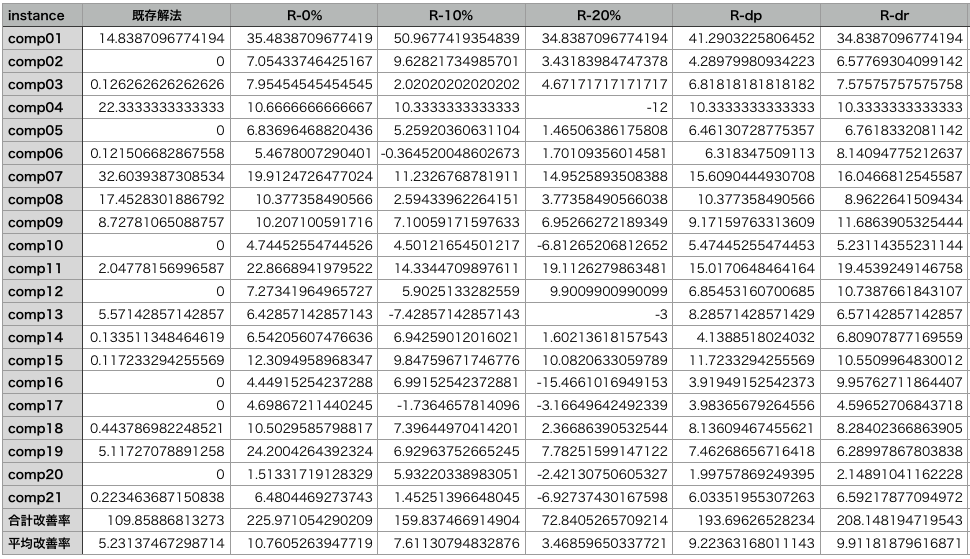
\includegraphics[width=12cm]{improve.png}
%\end{frame}
%
%\begin{frame}{初期解と既存の最良値を含めた比較}
%  \centering
% 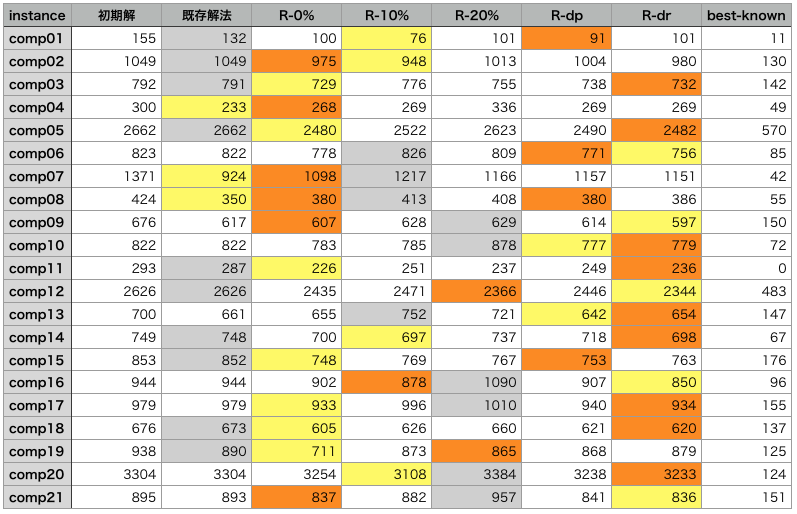
\includegraphics[width=12cm]{comp.png}
%\end{frame}
\backupend
\end{document}

%%% Local Variables:
%%% mode: latex
%%% TeX-master: t
%%% End:
